\documentclass[11pt]{article} \usepackage[top=2cm, bottom=2cm, left=2cm, right=2cm]{geometry}
\usepackage[francais]{babel} \usepackage{fontspec} % remplace \usepackage[utf8]{inputenc} et \usepackage[T1]{fontenc}
\usepackage{amsmath} \usepackage{amsfonts} \usepackage{amssymb} \usepackage{algorithm} \usepackage{algpseudocode}
\usepackage[babel=true]{csquotes} % csquotes va utiliser la langue définie dans babel

% ------------Raccourcis-------------
\newcommand{\abs}[1]{\left\lvert#1\right\rvert} \newcommand{\norm}[1]{\left\lVert#1\right\rVert}
\newcommand{\pars}[1]{\left(#1\right)} \newcommand{\bigpars}[1]{\bigl(#1\bigr)} \newcommand{\set}[1]{\left\{#1\right\}}
\newcommand{\floor}[1]{\lfloor #1 \rfloor} \newcommand{\ceil}[1]{\lceil #1 \rceil}



\title{ACVL} \title{Le problème du voyageur de commerce} \author{SALL Amadou \and PIGN\'E Quentin } \date{\today}
\begin{document}

\maketitle

\section{Structure de données}
Nous avons une structure de données modélisant les graphes. Cette structure utilise une liste de sommets, une liste
d'arcs et la fonction coût associé au graphe sous forme de matrice. Cette structure est nécessaire juste pour afficher
les graphes et vérifier leur complétude. Tous les algorithmes que nous avons implémenté n'utilisent que la matrice de
distance qui à elle seule définie le graphe.
\section{Algorithmes}

\subsection*{Floyd-Warshall}
$d^{k+1}(i,j)$ est le plus court chemin de $i$ à $j$ n'utilisant que les sommets $\set{1,\cdots,k+1}$ comme sommet
intermédiaires. Dès lors, il n'y a que deux cas possibles :
\begin{description}
    \item[on passe par le sommet $k+1$ :]  dans ce cas, il faut aller de $i$ à $k+1$ de façon optimale (coût
  $d^{k}(i,k+1)$) puis quitter $k+1$ pour aller jusqu'à $j$ de façon optimale aussi (coût $d^{k}(k+1,j)$)
\item[on ne passe pas par le sommet $k+1$ :] dans ce cas on a toujours un coût de $d^{k}(i,j)$
\end{description}
Ainsi on a la formule :
\begin{displaymath}
  d^{k+1}(i,j) = d^{k}(i,k+1) + d^{k}(k+1,j) 
\end{displaymath}
Nous fallant calculer la matrice des $d^{n}(i,j)$, le coeur de l'algorithme de Floyd-Warshall s'écrit :
  \begin{algorithmic}[]
   \For{$k \gets 1,n$}
       \For{$i \gets 1,n$}
           \For{$ \gets 1,n$}
           \State $ d^{k+1}(i,j) = d^{k}(i,k+1) + d^{k}(k+1,j) $
           \EndFor
       \EndFor
   \EndFor
  \end{algorithmic}
Ainsi l'algorithme de Floyd-Warshall a un coût de $O(n^3)$

\subsection*{\'Enumération}
Cette algorithme a un coût en $O(n!)$. En effet lors à l'étape $k$ on a $k-1$ choix. Pour faire donc les $n$ étapes, on
a un coût de $(n-1)!$. On  a aussi $n$ possibilités pour le choix d'un noeud de départ.
  \begin{figure}[ht]
\begin{center}
  
  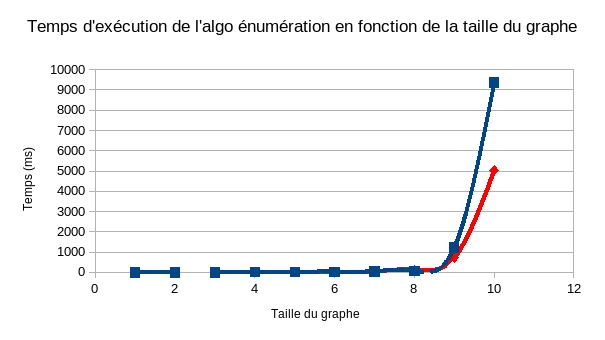
\includegraphics[scale=0.8]{images/exec_enum.png}
  \caption{Analyse de perfomances pour \'Enumération}
  \label{fig:enum}
\end{center}
\end{figure}
La figure \ref{fig:enum} montre que le temps d'execution de L'algorithme d'énumération est $O(n!)$
\subsection*{Algorithme glouton}
Il y a $n$ possibilités pour le choix du sommets de départ. Une fois le sommet de départ choisi (nommons le $i$) on choisit le sommet qui
minimise la distance. A l'étape $k$ on doit choisir entre $k-1$ sommets restants donc $k-1$ valeurs possibles, ce qui fait un coût de $k-1$. Au
total on a $O(\sum_{k=1}^{n-1} k)$ opérations. 
Ainsi l'algorithme glouton a un coût en $O(n^2)$
  \begin{figure}[ht]
\begin{center}
  
  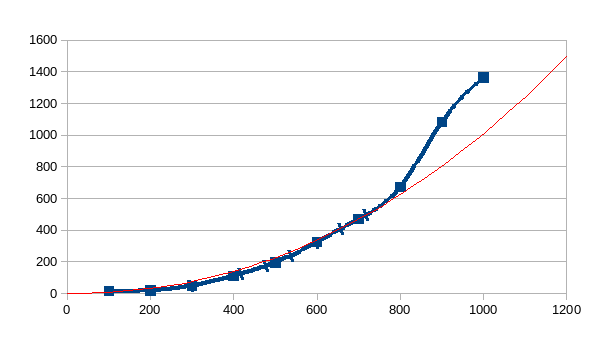
\includegraphics[scale=0.8]{images/exec_glouton.png}
  \caption{Analyse de perfomances pour L'algorithme glouton}
  \label{fig:glouton}
\end{center}
\end{figure}
\subsection*{Algorithme de recherche locale}
Pour un arc donné, disons $(u,v)$, le nombre d'arcs à tester est $n-4$. On a $n-1$ possibilités pour le choix de
$(u,v)$. Le coût de la recherche locale est donc $O(n^2)$. L'amélioration apportée par le recherche locale peut
atteindre plus de 50\%. Cependant on itère la recherche locale tant que c'est possible et rien ne ne garantit que, dans
le pire cas, on a pas un coût exponentiel. 
  \begin{figure}[ht]
\begin{center}
  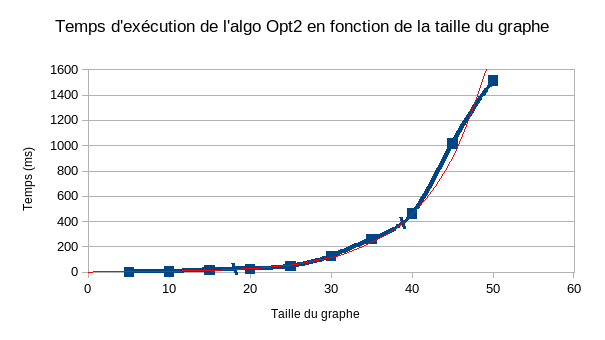
\includegraphics[scale=0.8]{images/exec_opt2.png}
  \caption{Analyse de perfomances pour 2-OPT}
  \label{fig:opt2}
\end{center}
\end{figure}
En tout cas, lorsque nous avons fait tourné l'algorithme, nous avons eu un
coût exponentiel (voir figure \ref{fig:opt2}). Sans doute sommes-nous tombés dans le pire cas.
\subsection*{Programmation dynamique}
Dans le chemin correspondant à $C(S,j)$ le prédécesseur $i_0$ de $j$ est l'un des $|S|-1$ éléments de
$\set{S} \backslash \set{j}$. Il faut arriver jusqu'à $i_0$ en passant par le plus court chemin utilisant une et une
seule fois les sommets de $\set{S} \backslash \set{j}$. Ainsi le coût est 
$C(\set{S} \backslash \set{j},i_0) + l_{(i_0,j)}$. Le $i_0$ correspondant est celui qui minimise la précédente somme car
sinon on serait passé par autre \enquote{prédécesseur potentiel} de $j$. Ainsi on a :
\begin{displaymath}
  C(S,j) = min_{i \in S , i \neq j}C(\set{S} \backslash \set{j},i)) + l_{(i,j)}
\end{displaymath}
La solution au problème est $C(E,n)$.
 Le nombre de sous-ensembles de $\set{1,\cdots,n}$ est $2^n$. Chacun de ces sous-ensembles contient $O(n)$ sommets. Pour
 un sommet $j$ de $S$, le calcul de $C(S,j)$ nécessite $O(n)$ opérations. 

Ainsi la programmation dynamique a un coût en $O(n^22^n)$

l'algorithme de programmation dynamique peut s'écrire :
%\begin{algorithm}[!ht]
%\caption{Programmation dynamique pour le TSP}
\begin{algorithmic}[]
%\Require une matrice de poids, un ensemble de $n$ sommets
\For{chaque sous-ensemble $S$ commençant par $1$}
\If{$|S| = 2$}
\For{$i$ de $1$ à $n$}
\State $C(S,i) \gets l_{(1,i)}$
\EndFor
\Else
\For{$i$ de $1$ à $n$}
\For{tous les $k$ $\notin$ $S - \{ 1 \}$}
\State $C(S,i) \gets \min$ $\{$ $C(S - \{ k \} ,k)$ + $l_{(k,i)}$ $\}$
\EndFor
\EndFor
\EndIf
\EndFor
\State retourner $\min$ $\{$ C(S,i) + $l_{(1,i)}$ $\}$ avec $|S| = $
(nombre de sommets - 1)
\end{algorithmic}
% \end{algorithm}

\section{Comparaison des algorithmes}
\begin{description}
    \item[Avantage de la programmation dynamique sur l'énumération :] les sous-chemins du circuit minimal sous aussi
  minimaux, on ne teste donc pas tous les circuits possibles. La complexité passe de $O(n!)$ à $O(n^22^n)$
  \item[Avantage de la combinaison glouton + recherche locale :] L'algorithme glouton permet de trouver des solutions en
des temps raisonnables. Cependant la valeur trouvée n'est pas forcément l'optimum. Appliquer L'algorithme de recherche
locale permet de gagner très nettement en précision (50\%)
\item[Glouton + recherche locale vs programmation dynamique :] La programmation dynamique est beaucoup plus précise mais
le coût en patît forcément. Juste le stockage de la matrice des stockage coute $O(n2^n)$

\end{description}

\end{document}